\section{Polarimeter Images}\label{sec:chp5-sec3}

As mentioned previously, the proposed polarimetric dermoscope is able to rotate the polarizer automatically in front of the camera at different angles.
In order to obtain the first three Stokes parameters, the polarizer is positioned automatically at the three angles of \ang{90}, \ang{45}, and \ang{0} with respect to the horizontal axis of the polarizer in front of the illumination system (\ac{psg}).
Using these angles, three images are acquired at each acquisition.
%In the first prototype 

The detector used by the dermoscope is Canon EOS 40D, with a 10.1 \si{\mega}\si{\px} \acf{cmos} sensor and acquires 14-bit raw images of size 3908 $\times$ 2602 \si{px}(1\si{px} $\approx$ 36 \si{\micro\meter}$^{2}$).
%Using the Schneide Componon-S 4.0/80 optical lense and magnfication of ratio 1, resolution of mm per pixel is achived.
The images are saved in Canon Raw-CR2 and \acs{jpeg} formats.
The left column in Fig.\,\ref{fig:DPex1} shows images of one series saved in \acs{jpeg} format.

\begin{figure}
	\begin{center}
		\captionsetup[subfigure]{labelformat=empty}
		\subfloat[\ang{90}]{\includegraphics[width = 0.45\textwidth]{Chapter5/Figures/IMG_6636.JPG}}\
		\subfloat[\ang{90}]{\includegraphics[width = 0.45\textwidth]{Chapter5/Figures/IMG_6636_png}}\\
		
		\subfloat[\ang{45}]{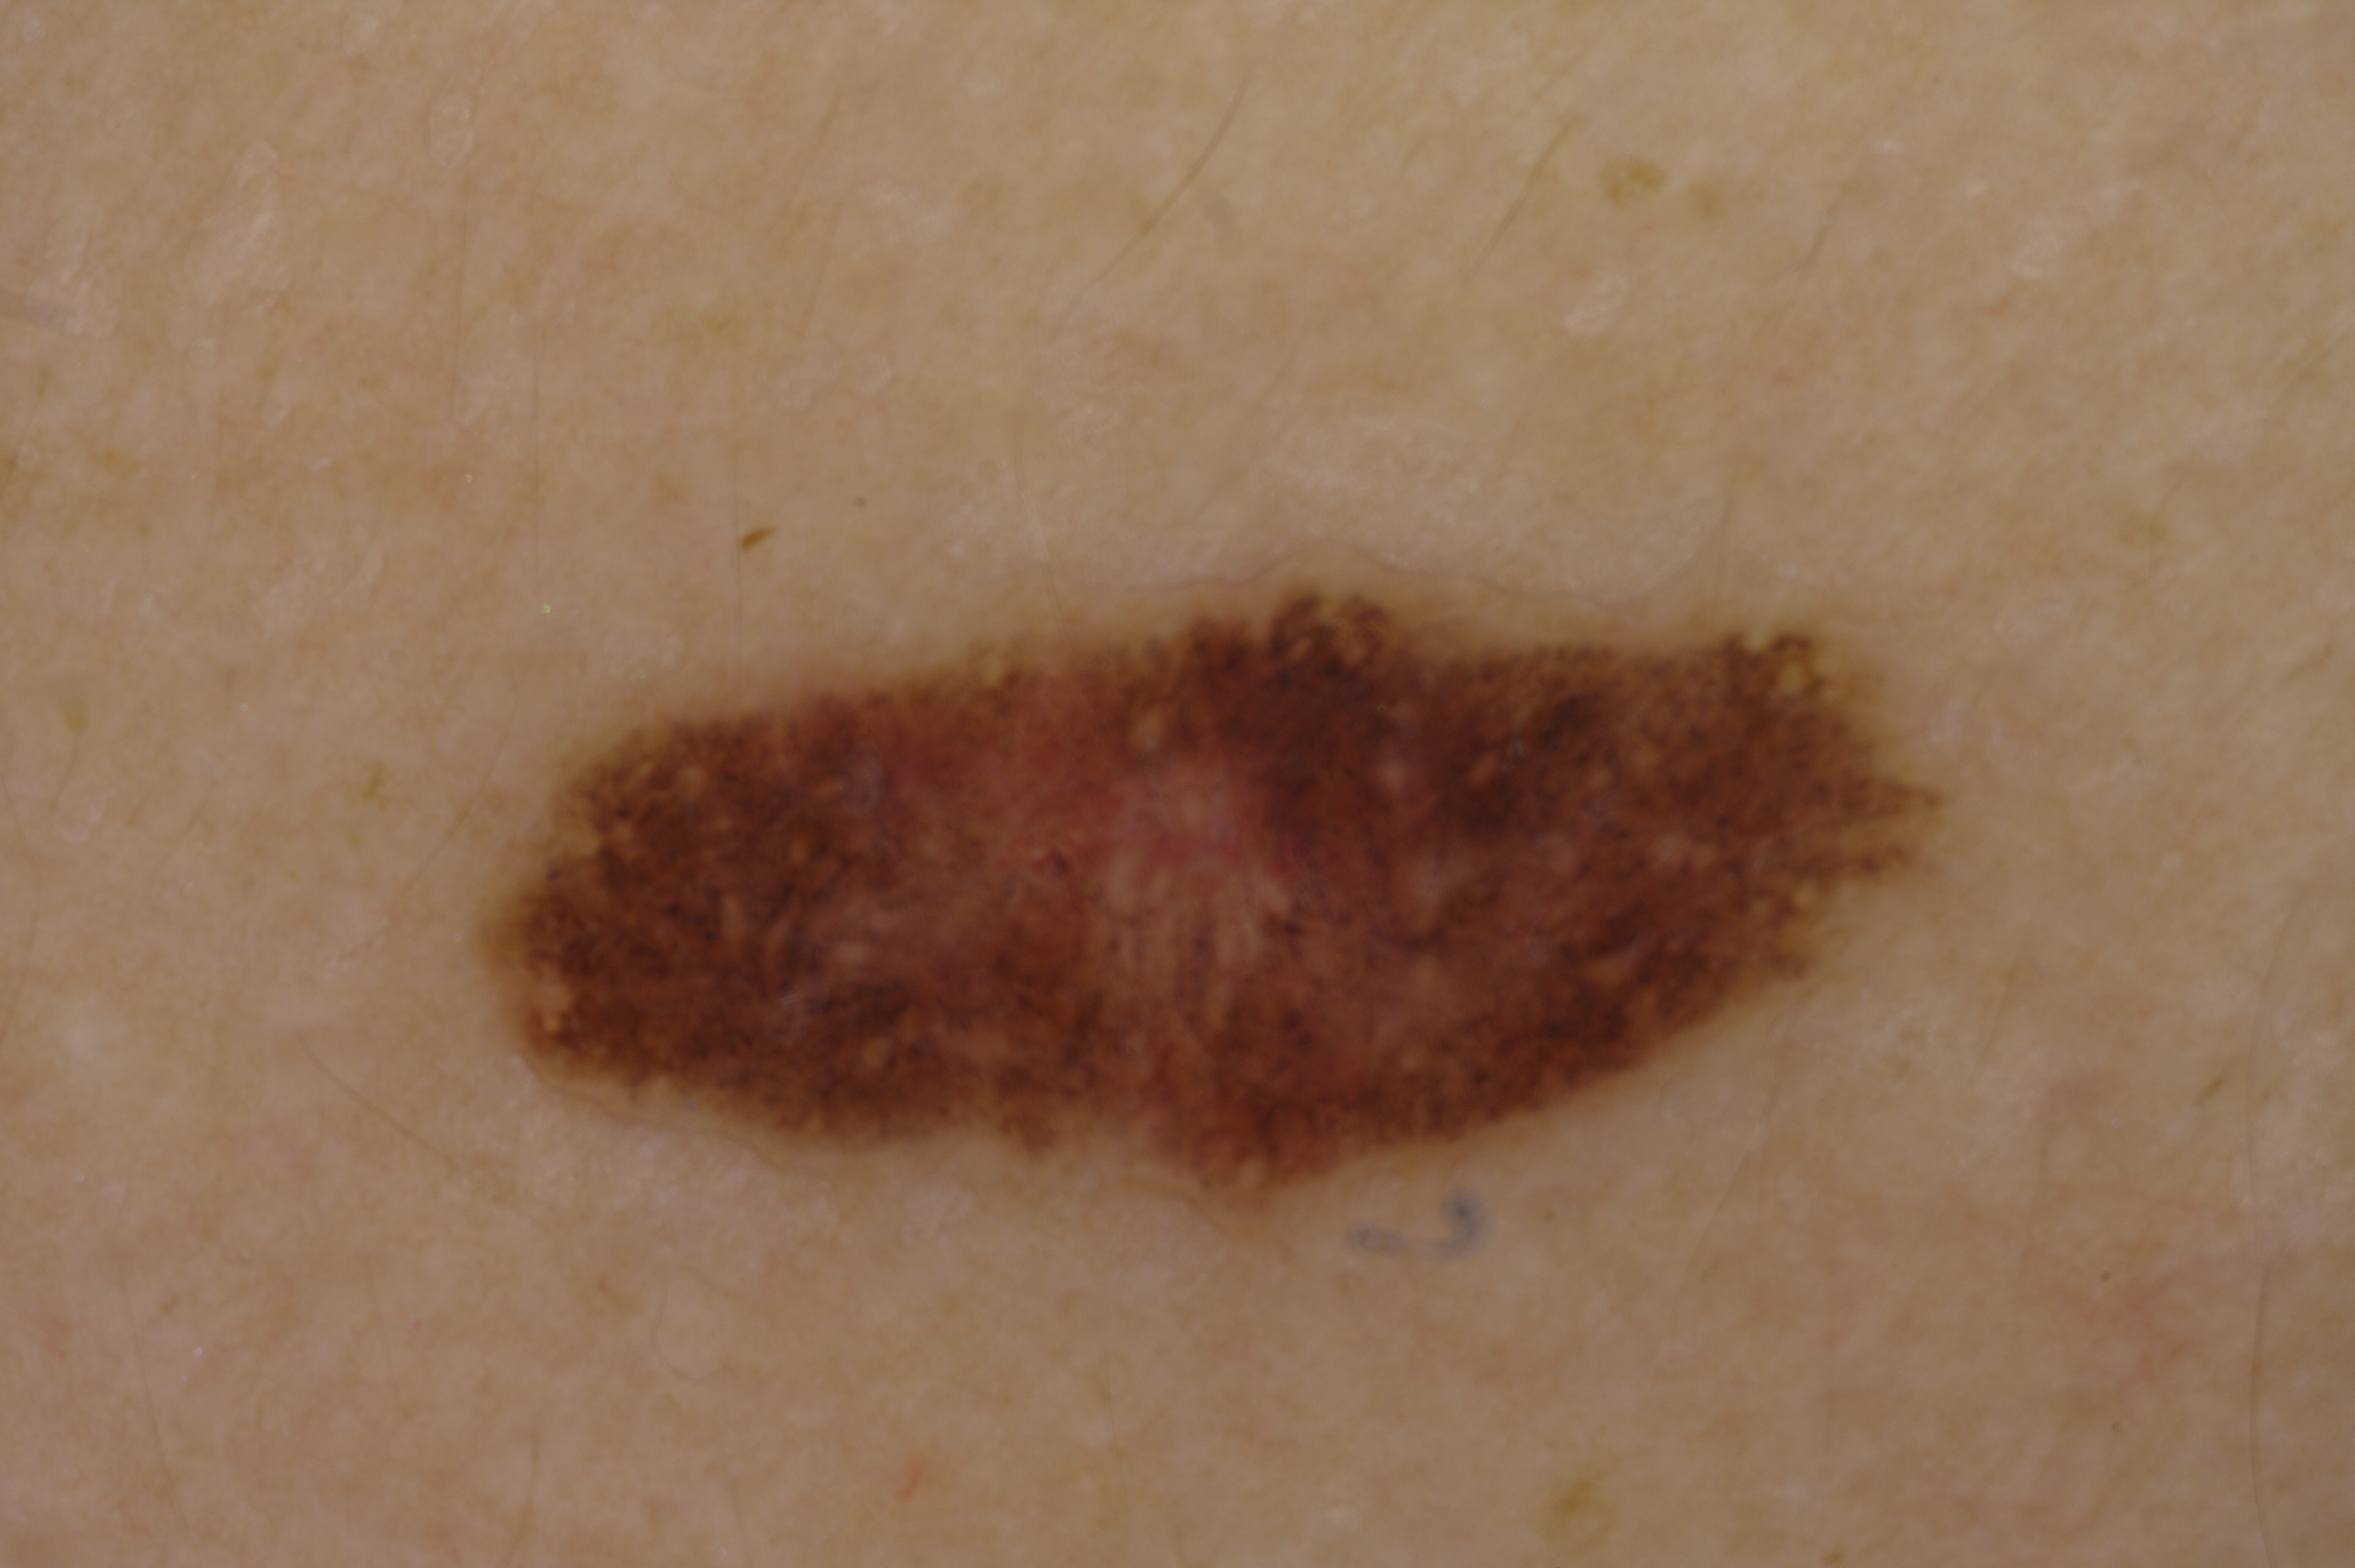
\includegraphics[width = 0.45\textwidth]{Chapter5/Figures/IMG_6637.JPG}}\
		\subfloat[\ang{45}]{\includegraphics[width = 0.45\textwidth]{Chapter5/Figures/IMG_6637_png.JPG}}\\
		
		\subfloat[\ang{0}]{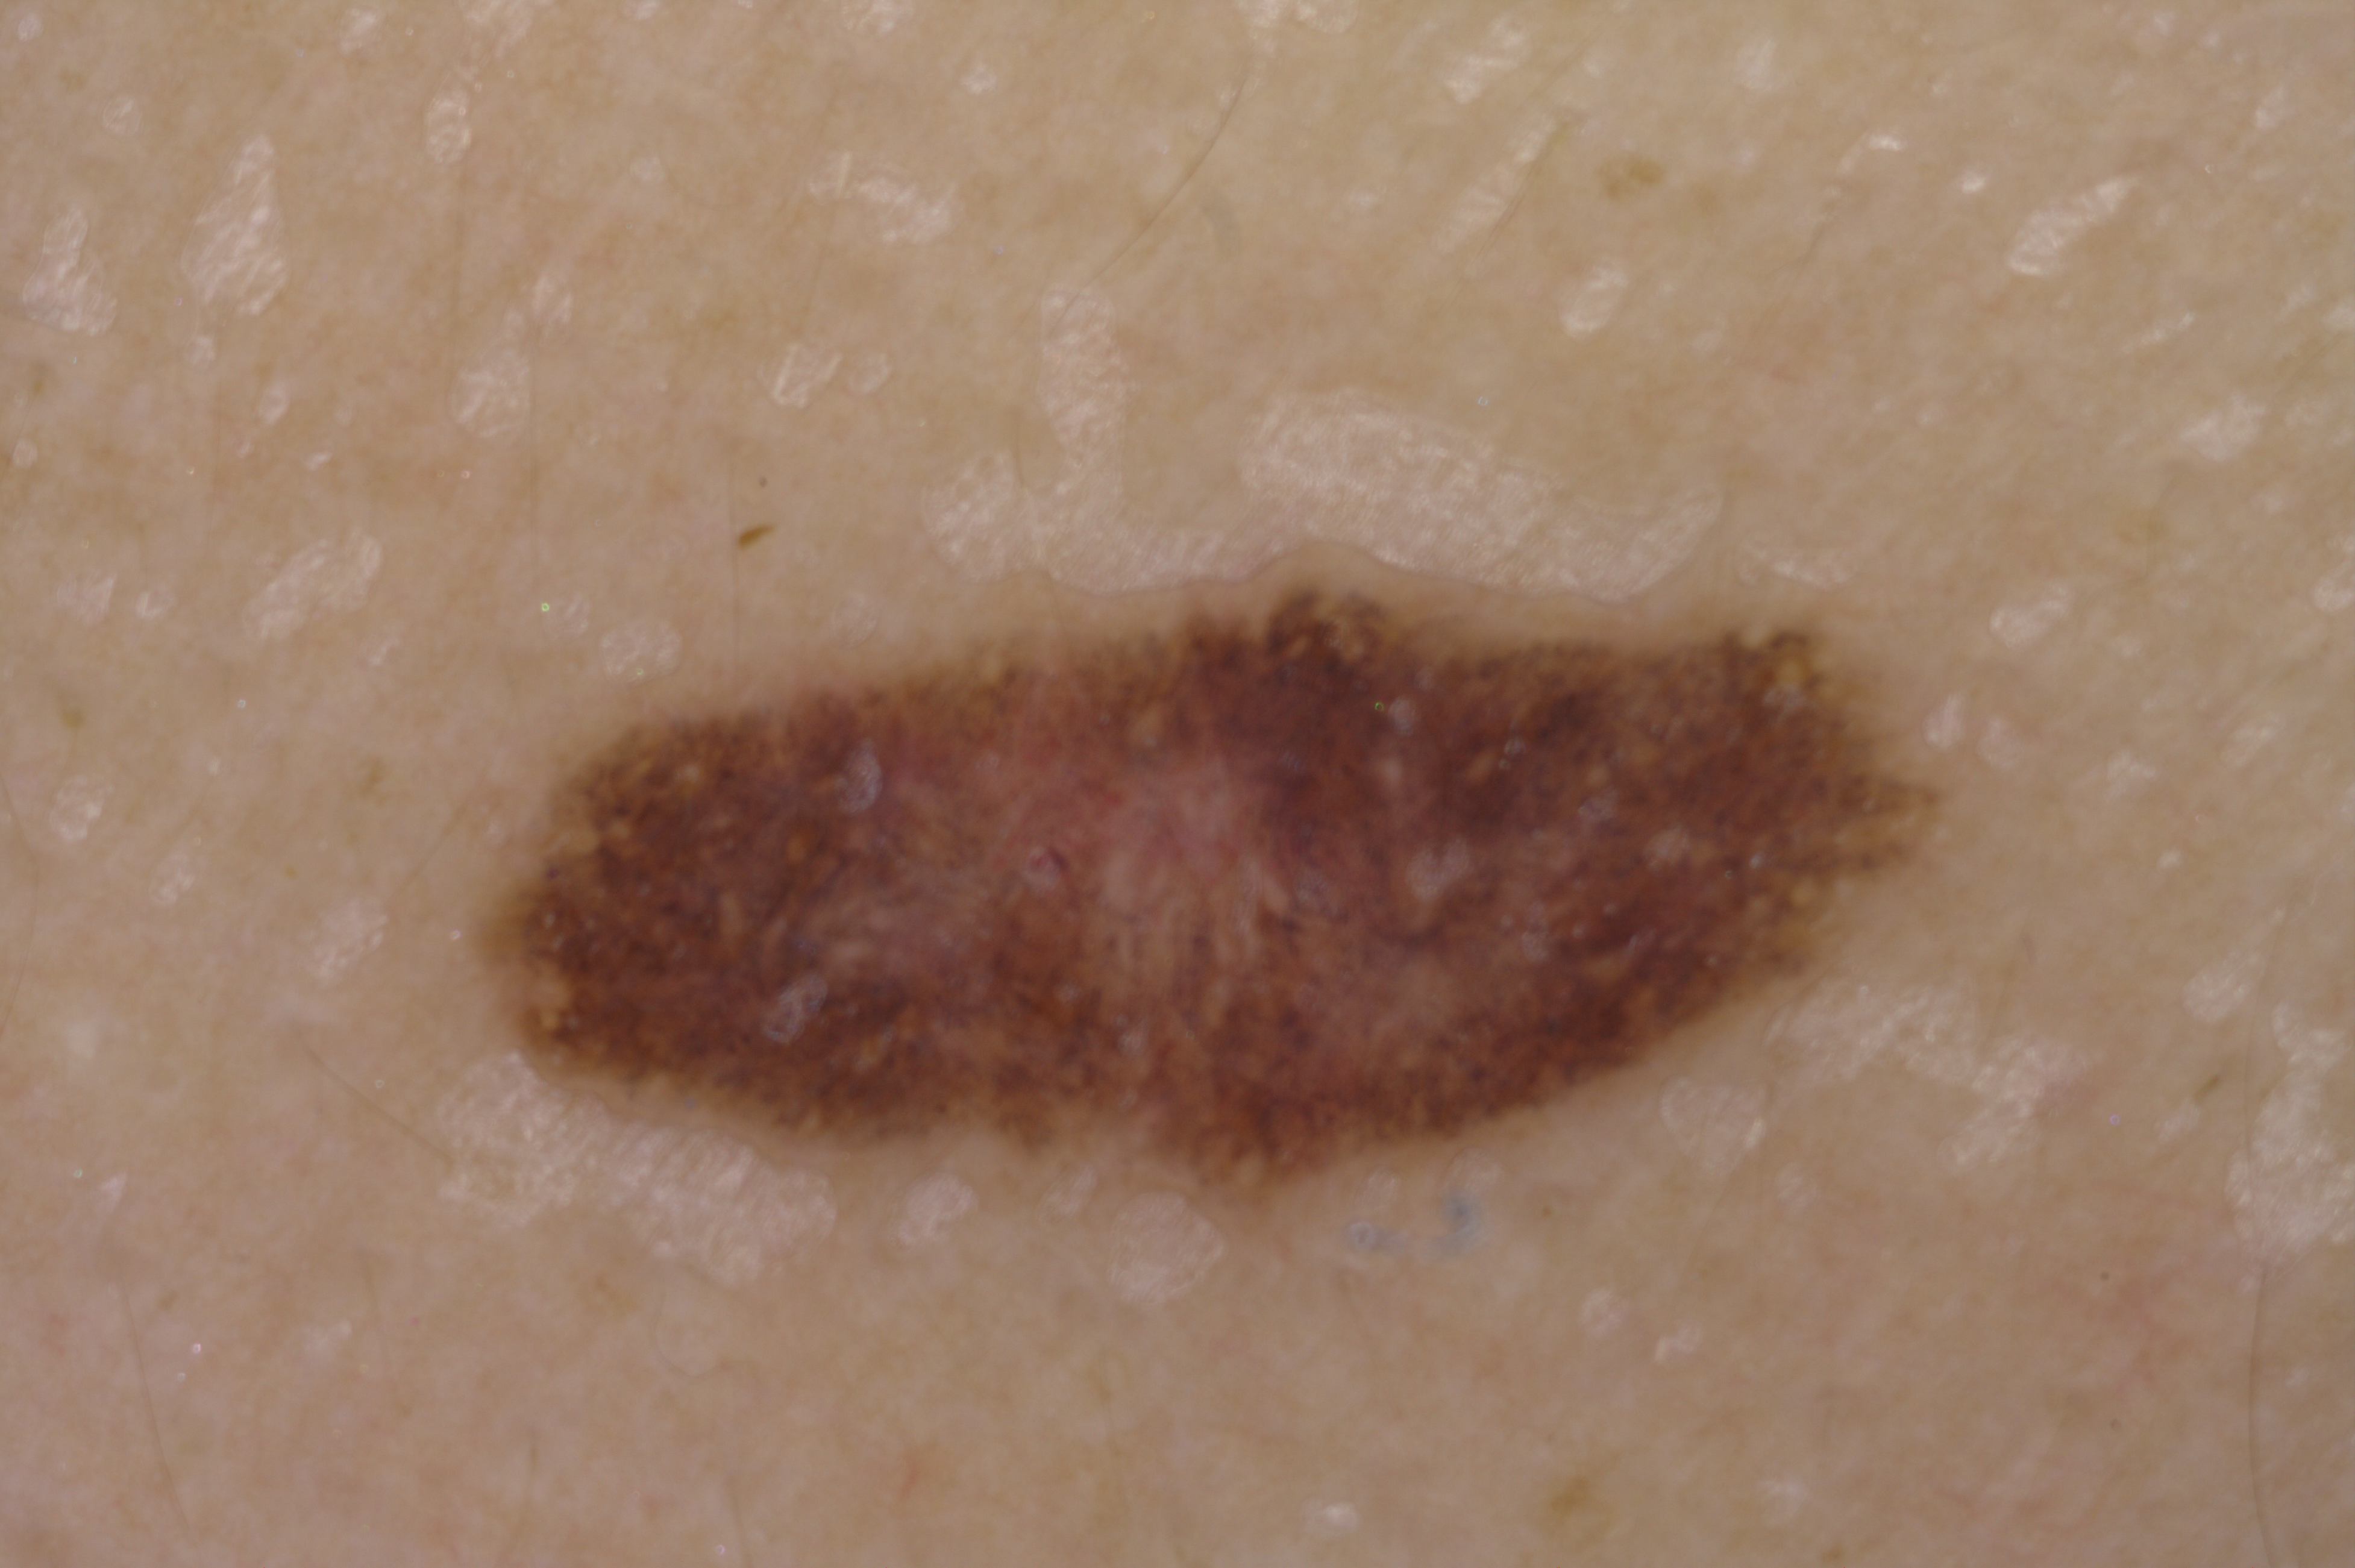
\includegraphics[width = 0.45\textwidth]{Chapter5/Figures/IMG_6638.JPG}}\
		\subfloat[\ang{0}]{\includegraphics[width = 0.45\textwidth]{Chapter5/Figures/IMG_6638_png.jpg}}	
		\end{center}
		\caption[Example of a polarimetric acquisition saved in \acs{jpeg} and sRGB images converted from Raw-CR2 to \acs{tiff}]{Example of a polarimetric acquisition. The left column shows images saved in \acs{jpeg} format and the right column illustrates sRGB \acs{tiff} images obtained from the conversion of Raw-CR2 images with the \ac{ufraw} software.
		Three images are acquired while the polarizer in the \acs{psa} unit is positioned at \ang{90}, \ang{45}, and \ang{0} with respect to the horizontal axis of the \acs{psg} polarizer.}
		\label{fig:DPex1}
\end{figure}

In polarization calculations, accurate original measurements are essential, so working with the raw data instead of \acs{jpeg} is required.
Thus, the RAW data are analyzed with the \acf{ufraw}\footnote{\url{http://ufraw.sourceforge.net/}} software.
This software uses DCRaw (David Coffin's)\footnote{\url{https://www.cybercom.net/~dcoffin/dcraw/}} conversion utility to read different Raw formats. 
In this research, the \ac{ufraw} software is applied to convert Raw-CR2 formats to standard-RGB (sRGB) color images.
The software uses camera white balance and a gamma correction of 0.45 without any further adjustment to convert Raw-CR2 to sRGB \acf{tiff} images.
The right column in Fig.\,\ref{fig:DPex1} shows the converted versions of the Raw-CR2 images.

As shown in Fig.\,\ref{fig:DPex1}, the specular reflections are removed when the \ac{psa} unit's polarizer is positioned at \ang{90} ($I_{\ang{90}}$, cross-polarized image) and are evident when the polarizer is positioned at \ang{0} ($I_{\ang{0}}$).
The three images acquired in each acquisition are used to compute the first three Stokes parameters (see Eq.\,\ref{Eq:cStokesmeas}).
%These parameters for the acquisition in Fig.\,\ref{fig:DP-ex1} are illustrated in Fig.\ref{fig:DP-ex1-S3}.
Prior to calculating the Stokes parameters, the three images are registered together. 
A detailed description of the registration step is given in Sect.\,\ref{sec:chp5-sec4}.
Due to the large size of the images, the Stokes parameters are calculated for a region of interest around each lesion.
\begin{figure}
	\begin{center}
		%\subfloat[I]{\includegraphics[width = 0.45\textwidth]{Chapter5/Figures/IMG_6636_I.jpg}}\\
		\subfloat[I~-~R]{\includegraphics[width = 0.45\textwidth]{Chapter5/Figures/IMG_6636_I_R_colorbar.jpg}}\hfill
		\subfloat[Q~-~R]{\includegraphics[width = 0.45\textwidth]{Chapter5/Figures/IMG_6636_Q_R_colorbar.jpg}}\\
                
                \subfloat[I~-~G]{\includegraphics[width = 0.45\textwidth]{Chapter5/Figures/IMG_6636_I_G_colorbar.jpg}}\hfill
		\subfloat[Q~-~G]{\includegraphics[width = 0.45\textwidth]{Chapter5/Figures/IMG_6636_Q_G_colorbar.jpg}}\\
		
		\subfloat[I~-~B]{\includegraphics[width = 0.45\textwidth]{Chapter5/Figures/IMG_6636_I_B_colorbar.jpg}}\hfill
                \subfloat[Q~-~B]{\includegraphics[width = 0.45\textwidth]{Chapter5/Figures/IMG_6636_Q_B_colorbar.jpg}}\\
                                
		\subfloat[I~-~Gray]{\includegraphics[width = 0.45\textwidth]{Chapter5/Figures/IMG_6636_I_Gray_colorbar.jpg}}\hfill
                \subfloat[Q~-~Gray]{\includegraphics[width = 0.45\textwidth]{Chapter5/Figures/IMG_6636_Q_Gray_colorbar.jpg}}
                
	\end{center}
	\caption[The first and second Stokes parameters, I, Q,  obtained from polarimetric images]{First and second Stokes parameters, I and Q in right and left columns, respectively, obtained from a polarimetric acquisition.}
	%	For the sake of visualization, the intensities in the second and third Stokes parameters (Q and U) are amplified 2 and 10 times, respectively.
	%	The illustrated lesion is a benign nevus.}
	\label{fig:Irgbgray}
\end{figure}

\begin{figure}
	\begin{center}
		\subfloat[U~-~R]{\includegraphics[width = 0.45\textwidth]{Chapter5/Figures/IMG_6636_U_R_colorbar.jpg}}\hfill
		\subfloat[U~-~G]{\includegraphics[width = 0.45\textwidth]{Chapter5/Figures/IMG_6636_U_G_colorbar.jpg}}\\
                \subfloat[U~-~B]{\includegraphics[width = 0.45\textwidth]{Chapter5/Figures/IMG_6636_U_B_colorbar.jpg}}\hfill
                \subfloat[U~-~Gray]{\includegraphics[width = 0.45\textwidth]{Chapter5/Figures/IMG_6636_U_Gray_colorbar.jpg}}
                
	\end{center}
	\caption[The third Stokes parameter, U,  obtained from polarimetric images]{Third Stokes parameters (U) obtained from a polarimetric acquisition.}
	\label{fig:Urgbgray}
\end{figure}

\begin{figure}
  \centering
  \subfloat[I~-~RGB]{\includegraphics[width= 0.45\textwidth]{Chapter5/Figures/IMG_6636_I.jpg}}\hfill
  \subfloat[Q~-~RGB]{\includegraphics[width= 0.45\textwidth]{Chapter5/Figures/IMG_6636_Q.jpg}}\
\caption[First and second Stokes parameters in RGB model.]{I and Q from Stokes parameters in RGB models.}
\label{fig:IQrgb}
\end{figure}

The first Stokes parameter, $I = HI = I_{\ang{0}} + I_{\ang{90}}$, adds the scattered light to the camera from the epidermis and papillary dermis ($I_{\ang{0}} = I_{\parallel}$) with the back-scattered light from the deeper layer of the dermis ($I_{\ang{90}} = I_{\perp}$).
Figure.\,\ref{fig:Irgbgray} showsn this parameter in R, G, B and gray channel.
The second Stokes parameter, $Q = HQ = I_{\ang{0}} - I_{\ang{90}}$, removes the light portion back-scattered from the deeper layer of dermis and only contains information from superficial layers (see Fig.\,\ref{fig:Irgbgray}, third and fourth rows).
The third Stokes parameter, $U = 2I_{\ang{45}} - I_{\ang{0}} - I_{\ang{90}}$, measures the difference between linearly \ang{45} and -\ang{45} polarized back-scattered light (see Fig.\,\ref{fig:Urgbgray}).
The perceived colors in the RGB representation of the first Stokes parameter, $I$, indicate that blue and green wavelengths are more absorbed by the melanin components in comparison with the red wavelength.
The bluish color in RGB representation of the Q image is evidence of the same fact and is due to the difference of blue intensities between $I_{\ang{0}}$ and $I_{\ang{90}}$, which is higher than the difference between red and green intensities (higher depolarization in blue channel).
Figure.\,\ref{fig:IQrgb} indicates these observations.

Using the Stokes parameters obtained, basic polarimetry properties, such as the \ac{dolp} and the \ac{aolp} can be obtained:
\begin{align}
\ac{dolp} & = \frac{(U^2 + Q^2)^{0.5}}{I},\\
\ac{aolp} & = 0.5*arctan2 (U,Q).
\label{eq:dolpaolp}
\end{align}
Figure~\ref{fig:dargb} and \ref{fig:dagray} illustrate the \ac{dolp} and \ac{aolp} in each color channel and grayscale. (the same lesion as in Fig.\,\ref{fig:DPex1}).
As shown in the second column in Fig.\,\ref{fig:dargb} and \ref{fig:dagray}, the \ac{aolp} has very low intensities (the angle is almost \ang{0}).
This is due to the construction and direction of the incident light.
Since the incident light is illuminated orthogonally to the skin, the majority of the reflected light is redirected in the same direction and the difference of the angle is very low.
%Due to this fact, for the sake of visualization, the intensities of the \ac{aolp} in Fig.\ref{fig:da-3c} are amplified three times.
% Why it is 0 most of the time ? 
The sample shown is a benign nevus, so for comparison, Figs.\,\ref{fig:S12melanoma1}, \ref{fig:damelanoma1}~\&~\ref{fig:S3melanoma1} show the first three Stokes parameters and the two polarization properties in R,G,B channels and grayscale for a melanoma sample, respectively.
%Using the images obtained from our first prototype, it was observed that there were no obvious sign of difference in polarized properties between melanoma and benign lesions. 

\begin{figure}
	\centering
	\subfloat[\ac{dolp}-R]{\includegraphics[width = 0.5 \textwidth, height = 0.25\textheight]{Chapter5/Figures/IMG_6636_DolpR_R_Colorbar2.eps}}\hfill
	\subfloat[\ac{aolp}-R]{\includegraphics[width = 0.5 \textwidth,  height = 0.25\textheight]{Chapter5/Figures/IMG_6636_AopR_R_Colorbar2.eps}}\\
	\subfloat[\ac{dolp}-G]{\includegraphics[width = 0.5 \textwidth,  height = 0.25\textheight]{Chapter5/Figures/IMG_6636_DolpR_G_Colorbar2.eps}}\hfill
	\subfloat[\ac{aolp}-G]{\includegraphics[width = 0.5 \textwidth,  height = 0.25\textheight]{Chapter5/Figures/IMG_6636_AopR_G_Colorbar2.eps}}\\
	\subfloat[\ac{dolp}-B]{\includegraphics[width = 0.5 \textwidth,  height = 0.25\textheight]{Chapter5/Figures/IMG_6636_DolpR_B_Colorbar2.eps}}\hfill
	\subfloat[\ac{aolp}-B]{\includegraphics[width = 0.5 \textwidth,  height = 0.25\textheight]{Chapter5/Figures/IMG_6636_AopR_B_Colorbar2.eps}}
	%\subfloat[]{\includegraphics[width = 0.4 \textwidth]{Chapter5/Figures/IMG_6636_DolpR.png}}\hfill
	%\subfloat[]{\includegraphics[width = 0.4 \textwidth]{Chapter5/Figures/IMG_6636_AopR3.png}}
	\caption[Degree of linear polarization (DOLP) and \ac{aolp} in the R,G, and B channels]{\ac{dolp} and \ac{aolp} obtained from I, Q, and U in the three color channels.}
	\label{fig:dargb}
\end{figure}

\clearpage

\begin{figure}
  \centering
	\subfloat[\ac{dolp}-Gray]{\includegraphics[width = 0.45 \textwidth]{Chapter5/Figures/IMG_6636_DoP_Gray_colorbar.jpg}}\hfill
	\subfloat[\ac{aolp}-Gray]{\includegraphics[width = 0.45 \textwidth]{Chapter5/Figures/IMG_6636_AoP_Gray_colorbar.jpg}}\\
        \caption[DOLP and \ac{aolp} in grayscale]{DOLP and AOLP obtained from mono-channel, grayscale of I$_{\ang{90}}$, I$_{\ang{45}}$, and I$_{\ang{0}}$.}
        \label{fig:dagray}
\end{figure}
\begin{figure}
	\centering
	\subfloat[I~-~R]{\includegraphics[width = 0.45\textwidth]{Chapter5/Figures/IMG_6561_I_R_colorbar.jpg}}\hfill
	\subfloat[Q~-~R]{\includegraphics[width = 0.45\textwidth]{Chapter5/Figures/IMG_6561_Q_R_colorbar.jpg}}\\
	\subfloat[I~-~G]{\includegraphics[width = 0.45\textwidth]{Chapter5/Figures/IMG_6561_I_G_colorbar.jpg}}\hfill
	\subfloat[Q~-~G]{\includegraphics[width = 0.45\textwidth]{Chapter5/Figures/IMG_6561_Q_G_colorbar.jpg}}\\
	\subfloat[I~-~B]{\includegraphics[width = 0.45\textwidth]{Chapter5/Figures/IMG_6561_I_B_colorbar.jpg}}\hfill
	\subfloat[Q~-~B]{\includegraphics[width = 0.45\textwidth]{Chapter5/Figures/IMG_6561_Q_B_colorbar.jpg}}\\
	\subfloat[I~-~Gray]{\includegraphics[width = 0.45\textwidth]{Chapter5/Figures/IMG_6561_I_Gray_colorbar.jpg}}\hfill
	\subfloat[Q~-~Gray]{\includegraphics[width = 0.45\textwidth]{Chapter5/Figures/IMG_6561_Q_Gray_colorbar.jpg}}\\
	\caption[The first and second Stokes parameters for melanoma nevi]{First and second Stokes parameters (I, Q) for a melanoma sample, right and left column respectively.}
	\label{fig:S12melanoma1}
\end{figure}

\begin{figure}
	\centering
	\subfloat[U~-~R]{\includegraphics[width = 0.45\textwidth]{Chapter5/Figures/IMG_6561_U_R_colorbar.jpg}}\
	\subfloat[U~-~G]{\includegraphics[width = 0.45\textwidth]{Chapter5/Figures/IMG_6561_U_G_colorbar.jpg}}\\
	\subfloat[U~-~B]{\includegraphics[width = 0.45\textwidth]{Chapter5/Figures/IMG_6561_U_B_colorbar.jpg}}\
	\subfloat[U~-~Gray]{\includegraphics[width = 0.45\textwidth]{Chapter5/Figures/IMG_6561_U_Gray_colorbar.jpg}}\\
	\caption[Third Stokes parameter for melanoma nevi]{Third Stokes parameter (U) for a melanoma sample.}
	\label{fig:S3melanoma1}
\end{figure}

\begin{figure}
	\centering
	\subfloat[\ac{dolp}-R]{\includegraphics[width = 0.5 \textwidth]{Chapter5/Figures/IMG_6561_DoP_R_colorbar.jpg}}
	\subfloat[\ac{aolp}-R]{\includegraphics[width = 0.5 \textwidth]{Chapter5/Figures/IMG_6561_AoP_R_colorbar.jpg}}\\
	\subfloat[\ac{dolp}-G]{\includegraphics[width = 0.5 \textwidth]{Chapter5/Figures/IMG_6561_DoP_G_colorbar.jpg}}\hfill
	\subfloat[\ac{aolp}-G]{\includegraphics[width = 0.5 \textwidth]{Chapter5/Figures/IMG_6561_AoP_G_colorbar.jpg}}\\
	\subfloat[\ac{dolp}-B]{\includegraphics[width = 0.5 \textwidth]{Chapter5/Figures/IMG_6561_DoP_B_colorbar.jpg}}\hfill
	\subfloat[\ac{aolp}-B]{\includegraphics[width = 0.5 \textwidth]{Chapter5/Figures/IMG_6561_AoP_B_colorbar.jpg}}\\
	\subfloat[\ac{dolp}-Gray]{\includegraphics[width = 0.5 \textwidth]{Chapter5/Figures/IMG_6561_DoP_Gray_colorbar.jpg}}\hfill
	\subfloat[\ac{aolp}-Gray]{\includegraphics[width = 0.5 \textwidth]{Chapter5/Figures/IMG_6561_AoP_Gray_colorbar.jpg}}\\

	%\subfloat[]{\includegraphics[width = 0.4 \textwidth]{Chapter5/Figures/IMG_6636_DolpR.png}}\hfill
	%\subfloat[]{\includegraphics[width = 0.4 \textwidth]{Chapter5/Figures/IMG_6636_AopR3.png}}
	\caption[Degree of linear polarization (DOLP) and \ac{aolp} in the R,G,B channels of melanoma nevus]{\ac{dolp} and \ac{aolp} obtained from I, Q, and U in the three color channels and grayscale.}
	\label{fig:damelanoma1}
\end{figure}


%\begin{figure}
%	\centering
%	\subfloat[I~-~R]{\includegraphics[width = 0.45\textwidth]{Chapter5/Figures/IMG_7029_I_R_colorbar.jpg}}\
%	\subfloat[Q~-~R]{\includegraphics[width = 0.45\textwidth]{Chapter5/Figures/IMG_7029_Q_R_colorbar.jpg}}\\
%	\subfloat[I~-~G]{\includegraphics[width = 0.45\textwidth]{Chapter5/Figures/IMG_7029_I_G_colorbar.jpg}}\
%	\subfloat[Q~-~G]{\includegraphics[width = 0.45\textwidth]{Chapter5/Figures/IMG_7029_Q_G_colorbar.jpg}}\\
%	\subfloat[I~-~B]{\includegraphics[width = 0.45\textwidth]{Chapter5/Figures/IMG_7029_I_B_colorbar.jpg}}\
%	\subfloat[Q~-~B]{\includegraphics[width = 0.45\textwidth]{Chapter5/Figures/IMG_7029_Q_B_colorbar.jpg}}\\
%	\subfloat[I~-~Gray]{\includegraphics[width = 0.5\textwidth]{Chapter5/Figures/IMG_7029_I_Gray_colorbar.jpg}}\hfill
%	\subfloat[Q~-~Gray]{\includegraphics[width = 0.5\textwidth]{Chapter5/Figures/IMG_7029_Q_Gray_colorbar.jpg}}\\
%	\caption[The first and second Stokes parameters for melanoma nevi]{First and second Stokes parameters (I, Q) for a melanoma sample two, right and left column respectively.}
%	\label{fig:S12-melanoma2}
%\end{figure}

%\begin{figure}
%	\centering
%	\subfloat[U~-~R]{\includegraphics[width = 0.45\textwidth, height = 0.23\textheight]{Chapter5/Figures/IMG_7029_U_R_colorbar.jpg}}\
%	\subfloat[U~-~G]{\includegraphics[width = 0.45\textwidth, height = 0.23\textheight]{Chapter5/Figures/IMG_7029_U_G_colorbar.jpg}}\\
%	\subfloat[U~-~B]{\includegraphics[width = 0.45\textwidth, height = 0.23\textheight]{Chapter5/Figures/IMG_7029_U_B_colorbar.jpg}}\
%	\subfloat[U~-~Gray]{\includegraphics[width = 0.5\textwidth, height = 0.23\textheight]{Chapter5/Figures/IMG_7029_U_Gray_colorbar.jpg}}\\
%	\caption[Third Stokes parameter for melanoma nevi]{Third Stokes parameter (U) for a melanoma sample Two.}
%	\label{fig:S3-melanoma2}
%\end{figure}

%\begin{figure}
%	\centering
%	\subfloat[\ac{dolp}-R]{\includegraphics[width = 0.5 \textwidth]{Chapter5/Figures/IMG_7029_DoP_R_colorbar.jpg}}
%	\subfloat[\ac{aolp}-R]{\includegraphics[width = 0.5 \textwidth]{Chapter5/Figures/IMG_7029_AoP_R_colorbar.jpg}}\\
%	\subfloat[\ac{dolp}-G]{\includegraphics[width = 0.5 \textwidth]{Chapter5/Figures/IMG_7029_DoP_G_colorbar.jpg}}\hfill
%	\subfloat[\ac{aolp}-G]{\includegraphics[width = 0.5 \textwidth]{Chapter5/Figures/IMG_7029_AoP_G_colorbar.jpg}}\\
%	\subfloat[\ac{dolp}-B]{\includegraphics[width = 0.5 \textwidth]{Chapter5/Figures/IMG_7029_DoP_B_colorbar.jpg}}\hfill
%	\subfloat[\ac{aolp}-B]{\includegraphics[width = 0.5 \textwidth]{Chapter5/Figures/IMG_7029_AoP_B_colorbar.jpg}}\\
%	\subfloat[\ac{dolp}-Gray]{\includegraphics[width = 0.5 \textwidth]{Chapter5/Figures/IMG_7029_DoP_Gray_colorbar.jpg}}\hfill
%	\subfloat[\ac{aolp}-Gray]{\includegraphics[width = 0.5 \textwidth]{Chapter5/Figures/IMG_7029_AoP_Gray_colorbar.jpg}}\\

%	%\subfloat[]{\includegraphics[width = 0.4 \textwidth]{Chapter5/Figures/IMG_6636_DolpR.png}}\hfill
%	%\subfloat[]{\includegraphics[width = 0.4 \textwidth]{Chapter5/Figures/IMG_6636_AopR3.png}}
%	\caption[Degree of linear polarization (DOLP) and \ac{aolp} in the R,G, and B channels- melanoma nevus]{\ac{dolp} and \ac{aolp} obtained from I, Q, and U in the three color channels and grayscale.}
%	\label{fig:da-melanoma2}
%\end{figure}


%\clearpage

%\clearpage
%\begin{figure}
%	\centering
%	\subfloat[\ac{dolp}]{\includegraphics[width = 0.45\textwidth, height = 0.25\textheight]{Chapter5/Figures/IMG_6561_DolpR_png.jpg}}\
%	\subfloat[\ac{dolp}]{\includegraphics[width = 0.45\textwidth, height = 0.25\textheight]{Chapter5/Figures/IMG_6890_DolpR_png.jpg}}\\
%	\subfloat[\ac{aolp}]{\includegraphics[width = 0.45\textwidth, height = 0.25\textheight]{Chapter5/Figures/IMG_6561_AopR_png.jpg}}\
%	\subfloat[\ac{aolp}]{\includegraphics[width = 0.45\textwidth, height = 0.25\textheight]{Chapter5/Figures/IMG_6890_AopR_png.jpg}}
%	\caption[Polarization properties: \ac{dolp}, and \ac{aolp} for a melanoma lesion]{Polarization properties: the \ac{dolp} and \ac{aolp} for two melanoma samples (left and right column, respectively). For visualization sake the intensities of \ac{aolp} intensities for two lesions are amplified 3 times.}
%	\label{fig:da-melanoma2}
%\end{figure}
%\clearpage
